\documentclass[12pt,a4paper]{article}
\usepackage[utf8]{vietnam}
\usepackage{amsmath}
\usepackage{amsfonts}
\usepackage{xcolor}
\usepackage{titlesec}
\usepackage{mdframed}
\usepackage{amssymb}
\usepackage{pgf,tikz,pgfplots}
\usepackage{graphicx}
\usepackage{cases} 
\pgfplotsset{compat=1.5}
\usepackage{mathrsfs}
\usetikzlibrary{arrows, calc}
\usepackage{float}
\usepackage{fancyhdr}
\pagestyle{fancy}
\pagestyle{empty}
\usepackage[left=2cm,right=2cm,top=2cm,bottom=2cm]{geometry}
\author{Nguyễn Văn Lộc}
\newmdenv[linecolor=black,skipabove=\topsep,skipbelow=\topsep,
leftmargin=-5pt,rightmargin=-5pt,
innerleftmargin=5pt,innerrightmargin=5pt]{mybox}
\begin{document}
\fancyhf{}
\lhead{}
\chead{}
\rhead{}
\cfoot{\thepage}
\rfoot{}
\lfoot{}
\pagestyle{fancy}
\renewcommand{\headrulewidth}{0pt}
\renewcommand{\footrulewidth}{0pt}
\begin{flushleft}
	\begin{mybox}
	\textbf{Họ và tên:} Nguyễn Văn Lộc\\
	\textbf{MSSV:} 20120131\\ 
	\textbf{Lớp:} 20CTT1TN\\
	\textbf{Ca:} Ca 1 sáng thứ 4
	\end{mybox}
\end{flushleft}
\begin{center}
	\textbf{BÀI TẬP THỰC HÀNH VI TÍCH PHÂN 2B}\\
	\textbf{CHƯƠNG 5: LÀM QUEN VÀI MÔ HÌNH PHƯƠNG TRÌNH VI PHÂN}
\end{center}
\textbf{Trang 85.}\\
\textbf{Bài 11.}
\begin{mybox}
Giải phương trình vi phân 
\begin{equation}
\frac{{dy}}{{dx}} = x{y^2}.
\label{eq1}
\end{equation}
\end{mybox}
Với \(y \ne 0,\) ta được phương trình (\ref{eq1}) tương đương với:
\[\frac{{dy}}{{{y^2}}} = xdx\]
\[ \Leftrightarrow \int {\frac{{dy}}{{{y^2}}} = \int {xdx} } \]
\[ \Leftrightarrow  - \frac{1}{y} = \frac{1}{2}{x^2} + C.\]
Xét tại \(y = 0.\) Do \(0' = {x^2} \cdot 0\) nên \(y = 0\) cũng là nghiệm của phương trình (\ref{eq1}).\\
Vậy phương trình (\ref{eq1}) có nghiệm là \(y = 0\) hoặc nghiệm thỏa mãn \(  - \frac{1}{y} = \frac{1}{2}{x^2} + C.\)\\
\textbf{Bài 14.}
\begin{mybox}
Giải phương trình vi phân
\begin{equation}
\left( {{y^2} + x{y^2}} \right)y' = 1.
\label{eq2}
\end{equation}
\end{mybox}
\begin{center}
(\ref{eq2}) \( \Leftrightarrow {y^2}\left( {1 + x} \right) \cdot \frac{{dy}}{{dx}} = 1\)
\end{center}
\[ \Leftrightarrow {y^2}dy = \frac{{dx}}{{x + 1}}\]
\[ \Leftrightarrow \int {{y^2}dy}  = \int {\frac{{dx}}{{x + 1}}} \]
\[ \Leftrightarrow \frac{1}{3}{y^3} = \ln \left| {x + 1} \right| + C.\]
\textbf{Bài 17.}
\begin{mybox}
Giải phương trình vi phân 
\begin{equation}
\frac{{dp}}{{dt}} = {t^2}p - p + {t^2} - 1.
\label{eq3}
\end{equation}
\end{mybox}
\begin{center}
(\ref{eq3}) \( \Leftrightarrow \frac{{dp}}{{dt}} = \left( {{t^2} - 1} \right)\left( {p + 1} \right)\)
\end{center}
Với \(p \ne  - 1,\) phương trình đã cho tương đương với
\[\frac{{dp}}{{p + 1}} = \left( {{t^2} - 1} \right)dt\]
\[ \Leftrightarrow \ln \left| {p + 1} \right| = \frac{1}{3}{t^3} - t + C.\]
Xét tại \(p = -1,\) do \({\left( { - 1} \right)^\prime } = \left( {{t^2} - 1} \right)\left( { - 1 + 1} \right)\) nên \(p = -1\) cũng là nghiệm của (\ref{eq3}).\\
Vậy phương trình (\ref{eq3}) có nghiệm là \(p = -1\) hoặc nghiệm thỏa mãn \(\ln \left| {p + 1} \right| = \frac{1}{3}{t^3} - t + C.\)\\
\textbf{Bài 28.}
\begin{mybox}
Tìm nghiệm của phương trình vi phân 
\begin{equation}
\label{eq4}
y'\tan x = a + y
\end{equation}
thỏa điều kiện \(y\left( {\frac{\pi }{3}} \right) = a\) với \(0 < x < \frac{\pi }{2}.\)
\end{mybox}
Với \(y \ne  - a,\) phương trình đã cho tương đương với
\[\frac{{dy}}{{a + y}} = \frac{{dx}}{{\tan x}}\]
\[ \Leftrightarrow \int {\frac{{dy}}{{a + y}} = \int {\frac{{dx}}{{\tan x}}} } \]
\[ \Leftrightarrow \ln \left| {y + a} \right| = \int {\frac{{\cos x}}{{\sin x}}dx} \]
\[ \Leftrightarrow \ln \left| {y + a} \right| = \ln \left| {\sin x} \right| + C\]
\[ \Leftrightarrow \ln \left| {y + a} \right| = \ln \left( {\sin x} \right) + C,\left( {0 < x < \frac{\pi }{2}} \right).\]
\[y\left( {\frac{\pi }{3}} \right) = a \Rightarrow \ln \left| {a + a} \right| = \ln \left( {\sin \left( {\frac{\pi }{3}} \right)} \right) + C\]
\[ \Rightarrow \ln 2 + \ln \left| a \right| = \frac{1}{2}\ln 3 - \ln 2 + C\]
\[ \Rightarrow C = \frac{1}{2}\ln 3 + 2\ln 2 + \ln \left| a \right|.\]
Xét \(y = -a,\) nghiệm này không thỏa mãn điều kiện đầu \(y\left( {\frac{\pi }{3}} \right) = a.\) \\
Vậy nghiệm của (\ref{eq4}) thỏa mãn \(\ln \left| {y + a} \right| = \ln \left( {\sin x} \right) + \frac{1}{2}\ln 3 + 2\ln 2 + \ln \left| a \right|.\)\\
\textbf{Bài 30.}
\begin{mybox}
Tìm nghiệm của phương trình vi phân 
\begin{equation}
\frac{{dy}}{{dx}} = \frac{x}{y}
\label{eq5}
\end{equation}
thỏa điều kiện \(y\left( 0 \right) =  - 3.\)
\end{mybox}
\begin{center}
(\ref{eq5}) \( \Leftrightarrow ydy = xdx\)
\end{center}
\[ \Leftrightarrow \int {ydy}  = \int {xdx} \]
\[ \Leftrightarrow \frac{1}{2}{y^2} = \frac{1}{2}{x^2} + {C_1}\]
\[ \Leftrightarrow {y^2} = {x^2} + C.\]
\[y\left( 0 \right) =  - 3 \Rightarrow 9 = 0 + C \Rightarrow C = 9.\]
\[ \Rightarrow {y^2} = {x^2} + 9\]
\[ \Leftrightarrow \left[ \begin{gathered}
  y = \sqrt {{x^2} + 9}  \hfill \\
  y =  - \sqrt {{x^2} + 9}  \hfill \\ 
\end{gathered}  \right..\]
Do \(y\left( 0 \right) =  - 3 < 0\) nên ta chọn nghiệm \(y =  - \sqrt {{x^2} + 9} .\)\\
\textbf{Bài 33.}
\begin{mybox}
Tìm nghiệm của phương trình vi phân 
\begin{equation}
\frac{{dL}}{{dt}} = k{L^2}\ln t
\label{eq6}
\end{equation}
thỏa điều kiện \(L\left( 1 \right) =  - 1.\)
\end{mybox}
Với \(L \ne 0,\) phương trình đã cho tương đương với
\[\frac{{dL}}{{{L^2}}} = k\ln tdt\]
\[ \Leftrightarrow \int {\frac{{dL}}{{{L^2}}}}  = k\int {\ln tdt} \]
\begin{equation}
\Leftrightarrow  - \frac{1}{L} = k\int {\ln tdt} 
\label{eq7}
\end{equation}
Đặt \(\left\{ \begin{gathered}
  u = \ln t \hfill \\
  dv = dt \hfill \\ 
\end{gathered}  \right. \Rightarrow \left\{ \begin{gathered}
  du = \frac{1}{t}dt \hfill \\
  v = t \hfill \\ 
\end{gathered}  \right..\)
\[ \Rightarrow \int {\ln tdt}  = t \cdot \ln t - \int {\frac{1}{t} \cdot tdt} \]
\[ \Rightarrow \int {\ln tdt}  = t\ln t - \int {1dt} \]
\[ \Rightarrow \int {\ln tdt}  = t\ln t - t + C.\]
Do đó,
\begin{center}
(\ref{eq7}) \( \Leftrightarrow  - \frac{1}{L} = k\left( {t\ln t - t + C} \right).\)
\end{center}
\[L\left( 1 \right) =  - 1 \Rightarrow 1 = k\left( {C - 1} \right)\]
\[ \Rightarrow C = \frac{1}{k} + 1 = \frac{{k + 1}}{k}.\]
Vì vậy,
\[ - \frac{1}{L} = k\left( {t\ln t - t + \frac{{k + 1}}{k}} \right)\]
\[ \Leftrightarrow  - \frac{1}{L} = kt\ln t - kt + k + 1.\]
Xét \(L = 0,\) nghiệm này không thỏa mãn điều kiện đầu \(L\left( 1 \right) =  - 1.\)\\
Vậy nghiệm của (\ref{eq6}) thỏa mãn \( - \frac{1}{L} = kt\ln t - kt + k + 1.\)\\
\textbf{Trang 87.}\\
\textbf{Bài 11.}
\begin{mybox}
Giải phương trình vi phân
\begin{equation}
y'\sin x + y\cos x = \sin \left( {{x^2}} \right).
\label{eq8}
\end{equation}
\end{mybox}
\begin{center}
(\ref{eq8}) \( \Leftrightarrow {\left( {y\sin x} \right)^\prime } = \sin \left( {{x^2}} \right)\)
\end{center}
\[ \Leftrightarrow y\sin x = \int {\sin \left( {{x^2}} \right)} dx\]
\[y = \frac{1}{{\sin x}}\left( {C + \int\limits_a^x {\sin \left( {{x^2}} \right)dx} } \right)\]
\textbf{Bài 13.}
\begin{mybox}
Giải phương trình vi phân
\begin{equation}
\left( {1 + t} \right)\frac{{du}}{{dt}} + u = 1 + t, t > 0.
\label{eq9}
\end{equation}
\end{mybox}
\begin{center}
(\ref{eq9}) \( \Leftrightarrow {\left[ {u \cdot \left( {t + 1} \right)} \right]^\prime } = \left( {1 + t} \right)\)
\end{center}
\[ \Leftrightarrow u \cdot \left( {t + 1} \right) = \int {\left( {1 + t} \right)dt} \]
\[ \Leftrightarrow u \cdot \left( {t + 1} \right) = \frac{1}{2}{t^2} + t + C.\]
\textbf{Bài 15.}
\begin{mybox}
Giải phương trình vi phân
\begin{equation}
y' - y = e^x.
\label{eq10}
\end{equation}
\end{mybox}
\begin{center}
(\ref{eq10}) \( \Leftrightarrow y'{e^{ - x}} - y{e^{ - x}} = 1\)
\end{center}
\[ \Leftrightarrow {\left( {y \cdot {e^{ - x}}} \right)^\prime } = 1\]
\[ \Leftrightarrow y{e^{ - x}} = \int {1dx} \]
\[ \Leftrightarrow y{e^{ - x}} = x + C\]
\textbf{Bài 17.}
\begin{mybox}
Giải phương trình vi phân
\begin{equation}
4{x^3}y + {x^4}y' = {\sin ^3}x.
\label{eq11}
\end{equation}
\end{mybox}
\begin{center}
(\ref{eq11}) \( \Leftrightarrow {\left( {{x^4}y} \right)^\prime } = {\sin ^3}x\)
\end{center}
\[ \Leftrightarrow {x^4}y = \int {{{\sin }^3}xdx} \]
\[ \Leftrightarrow {x^4}y = \int {{{\sin }^2}x\sin xdx} \]
\[ \Leftrightarrow {x^4}y =  - \int {\left( {1 - {{\cos }^2}x} \right)} d\left( {\cos x} \right)\]
\[ \Leftrightarrow {x^4}y = \int {\left( {{{\cos }^2}x - 1} \right)d\left( {\cos x} \right)} \]
\[ \Leftrightarrow {x^4}y = \frac{1}{3}{\cos ^3}x - \cos x + C.\]
\textbf{Bài 22.}
\begin{mybox}
Giải phương trình vi phân
\begin{equation}
t\ln t\frac{{dr}}{{dt}} + r = t{e^t}.
\label{eq12}
\end{equation}
\end{mybox}
\begin{center}
(\ref{eq12}) \( \Leftrightarrow \frac{{dr}}{{dt}} + \frac{r}{{t\ln t}} = \frac{{{e^t}}}{{\ln t}}\)
\end{center}
\[ \Leftrightarrow \frac{{dr}}{{dt}} \cdot {e^{\int {\frac{1}{{t\ln t}}dt} }} + \frac{r}{{t\ln t}} \cdot {e^{\int {\frac{1}{{t\ln t}}dt} }} = \frac{{{e^t}}}{{\ln t}} \cdot {e^{\int {\frac{1}{{t\ln t}}dt} }}\]
\[ \Leftrightarrow \frac{{dr}}{{dt}} \cdot {e^{\ln \left( {\left| {\ln t} \right|} \right)}} + \frac{r}{{t\ln t}} \cdot {e^{\ln \left( {\left| {\ln t} \right|} \right)}} = \frac{{{e^t}}}{{\ln t}} \cdot {e^{\ln \left( {\left| {\ln t} \right|} \right)}}\]
\begin{equation}
\label{eq13}
\Leftrightarrow \frac{{dr}}{{dt}}\left| {\ln t} \right| + \frac{r}{{t\ln t}} \cdot \left| {\ln t} \right| = \frac{{{e^t}}}{{\ln t}} \cdot \left| {\ln t} \right|.
\end{equation}
Khi \(\ln t > 0,\)
\begin{center}
(\ref{eq13}) \( \Leftrightarrow \frac{{dr}}{{dt}}\ln t + \frac{r}{t} = {e^t}.\)
\end{center}
Khi \(\ln t < 0,\)
\begin{center}
(\ref{eq13}) \( \Leftrightarrow \frac{{dr}}{{dt}}\left( { - \ln t} \right) - \frac{r}{t} =  - {e^t}\)
\end{center}
\[ \Leftrightarrow \frac{{dr}}{{dt}}\ln t + \frac{r}{t} = {e^t}.\]
Vậy phương trình (\ref{eq13}) tương đương với
\[\frac{{dr}}{{dt}}\ln t + \frac{r}{t} = {e^t}.\]
\[ \Leftrightarrow {\left( {r\ln t} \right)^\prime } = {e^t}\]
\[ \Leftrightarrow r\ln t = \int {{e^t}dt} \]
\[ \Leftrightarrow r\ln t = {e^t} + C.\]
\textbf{Trang 88.}\\
\textbf{Bài 30.}
\begin{mybox}
Giải bài toán giá trị đầu
\begin{equation}
xy' = y + {x^2}\sin x,
\label{eq14}
\end{equation}
với \(y\left( \pi  \right) = 0.\)
\end{mybox}
\begin{center}
(\ref{eq14}) \( \Leftrightarrow xy' - y = {x^2}\sin x\)
\end{center}
\[ \Leftrightarrow y' - \frac{y}{x} = x\sin x\]
\[ \Leftrightarrow y' \cdot {e^{ - \ln \left| x \right|}} - \frac{y}{x}{e^{ - \ln \left| x \right|}} = x{e^{ - \ln \left| x \right|}}\sin x\]
\begin{equation}
 \label{eq15}
 \Leftrightarrow y' \cdot \frac{1}{{\left| x \right|}} - \frac{y}{x} \cdot \frac{1}{{\left| x \right|}} = x \cdot \frac{1}{{\left| x \right|}}\sin x.
\end{equation}
Khi \(x > 0,\) 
\begin{center}
(\ref{eq15}) \( \Leftrightarrow \frac{{y'}}{x} - \frac{y}{{{x^2}}} = \sin x.\)
\end{center}
Khi \(x < 0,\)
\begin{center}
(\ref{eq15}) \( \Leftrightarrow  - \frac{{y'}}{x} + \frac{y}{{{x^2}}} =  - \sin x\)
\end{center}
\[ \Leftrightarrow \frac{{y'}}{x} - \frac{y}{{{x^2}}} = \sin x.\]
Vậy phương trình (\ref{eq15}) tương đương với
\[\frac{{y'}}{x} - \frac{y}{{{x^2}}} = \sin x.\]
\[ \Leftrightarrow {\left( {\frac{y}{x}} \right)^\prime } = \sin x\]
\[ \Leftrightarrow \frac{y}{x} = \int {\sin xdx} \]
\[ \Leftrightarrow \frac{y}{x} =  - \cos x + C\]
\[y\left( \pi  \right) = 0 \Rightarrow 0 =  - \cos \pi  + C \Rightarrow C =  - 1.\]
Khi đó
\[\frac{y}{x} =  - \cos x - 1\]
\[ \Leftrightarrow y =  - x\cos x - x.\]
\textbf{Bài 32.}
\begin{mybox}
Giải bài toán giá trị đầu
\begin{equation}
{x^2}y' + 2xy = \ln x,
\label{eq16}
\end{equation}
với \(y\left( 1 \right) = 2.\)
\end{mybox}
\begin{center}
(\ref{eq16}) \( \Leftrightarrow {\left( {{x^2}y} \right)^\prime } = \ln x\)
\end{center}
\[ \Leftrightarrow {x^2}y = \int {\ln xdx} \]
\[ \Leftrightarrow {x^2}y = x\ln x - x + C.\]
\[y\left( 1 \right) = 2 \Rightarrow 2 =  - 1 + C \Rightarrow C = 3.\]
Khi đó
\[{x^2}y = x\ln x - x + 3\]
\[ \Leftrightarrow y = \frac{{\ln x}}{x} - \frac{1}{x} + \frac{3}{{{x^2}}}.\]
\textbf{Trang 89}\\
\textbf{Bài 3.} (mô hình nhập vốn lãi liên tục)
\begin{mybox}
Một tài khoản có lượng tiền ban đầu là \(P\) (gốc). Lãi suất theo thời gian là \(r/\)năm, thường được viết ở dạng phần trăm/năm. Chẳng hạn \(r = 0.05 = 5\%\) có nghĩa là sau \(1\) năm thì cứ \(100\) đơn vị tiền tài khoản sẽ nhận được một khoản lãi là \(5\) đơn vị tiền. Nếu lãi được nhập vào vốn, thì \(r\) chính là tốc độ tăng tương đối của lượng tiền trong tài khoản. Trong mô hình nhập vốn lãi liên tục thì lượng tiền \(A\) ở thời điểm \(t\) (tính bằng năm) thỏa
\begin{equation}
\frac{{A'\left( t \right)}}{{A\left( t \right)}} = r.
\label{eq17}
\end{equation}
a. Chứng tỏ lượng tiền trong tài khoản được cho bởi
\[A\left( t \right) = P{e^{rt}}.\]
b. Chứng tỏ thời gian cần để lượng tiền trong tài khoản tăng gấp đôi không phụ thuộc vào khoản đầu tư ban đầu.\\
c. Để lượng tiền tăng gấp đôi mỗi \(10\) năm thì lãi suất phải bằng bao nhiêu?
\end{mybox}
a. 
\begin{center}
(\ref{eq17}) \( \Leftrightarrow A'\left( t \right) - rA\left( t \right) = 0\)
\end{center}
\[ \Leftrightarrow A'\left( t \right){e^{ - rt}} - r{e^{ - rt}}A\left( t \right) = 0\]
\[ \Leftrightarrow {\left[ {A\left( t \right){e^{ - rt}}} \right]^\prime } = 0\]
\[ \Leftrightarrow A\left( t \right){e^{ - rt}} = C\]
\[ \Leftrightarrow A\left( t \right) = C{e^{rt}}.\]
\[A\left( 0 \right) = P \Rightarrow P = C \cdot {e^0} \Rightarrow C = P.\]
\[ \Rightarrow A\left( t \right) = P{e^{rt}}.\]
b. Giả sử lượng tiền tại thời điểm \(t_2\) là gấp đôi lượng tiền tại thời điểm \(t_1.\)
\[ \Leftrightarrow A\left( {{t_2}} \right) = 2A\left( {{t_1}} \right)\]
\[ \Leftrightarrow P{e^{r{t_2}}} = 2P{e^{r{t_1}}}\]
\[ \Leftrightarrow {e^{r{t_2}}} = 2{e^{r{t_1}}}\]
\[ \Leftrightarrow r{t_2} = \ln 2 + r{t_1}\]
\[ \Leftrightarrow r\left( {{t_2} - {t_1}} \right) = \ln 2\]
\[ \Leftrightarrow {t_2} - {t_1} = \frac{{\ln 2}}{r}.\]
Vậy thời gian để lượng tiền trong tài khoản tăng gấp đôi không phụ thuộc vào khoản đầu tư ban đầu.\\
c. Lượng tiền tăng gấp đôi mỗi \(10\) năm
\[ \Leftrightarrow 10 = \frac{{\ln 2}}{r}\]
\[ \Leftrightarrow r = \frac{{\ln 2}}{{10}} \approx 0.07.\]
Vậy để lượng tiền tăng gấp đôi mỗi \(10\) năm thì lãi suất phải vào khoảng \(7 \%\)/năm.
\textbf{Trang 90.}\\
\textbf{Bài 9.}
\begin{mybox}
Hình dưới đây là một sơ đồ mạch điện đơn giản
\begin{figure}[H]
\center{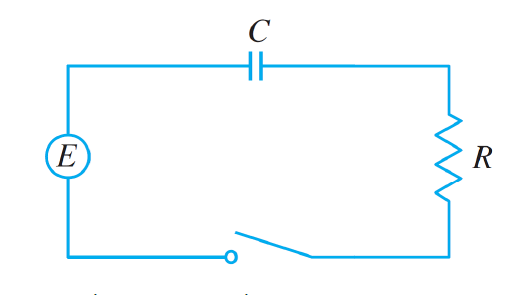
\includegraphics[scale=0.5]{c5_1}}
\end{figure}
trong đó gồm một nguồn phát điện, một tụ điện có điện dung \(C\) Farads (F), một điện trở có trở kháng \(R\) Ohms \(\left( \Omega  \right).\) Hiệu điện thế ở hai đầu tụ là \(\frac{Q}{C},\) trong đó \(Q\) là điện lượng (đơn vị Coulombs). Định luật Kirchhoff cho \(RI + \frac{Q}{C} = E\left( t \right).\) Nhưng \(I = \frac{{dQ}}{{dt}},\) do đó ta có
\begin{equation}
R\frac{{dQ}}{{dt}} + \frac{1}{C}Q = E\left( t \right)
\label{eq18}
\end{equation}
Giả sử \(R = 5\Omega ,\) điện dung là \(C = 0.05F\) và pin cấp điện năng \(60V,\) điện lượng lúc đầu \(C = 0.05F.\) Tìm điện lượng trong tụ ở thời điểm \(t.\)
\end{mybox}
Thay các số liệu đã cho vào phương trình (\ref{eq18}), ta được
\[5\frac{{dQ}}{{dt}} + 20Q = 60\]
\[ \Leftrightarrow \frac{{dQ}}{{dt}} + 4Q = 12\]
\[ \Leftrightarrow \frac{{dQ}}{{dt}} \cdot {e^{4t}} + 4{e^{4t}}Q = 12{e^{4t}}\]
\[ \Leftrightarrow {\left( {{e^{4t}} \cdot Q} \right)^\prime } = 12{e^{4t}}\]
\[ \Leftrightarrow {e^{4t}} \cdot Q = \int {12{e^{4t}}dt} \]
\[ \Leftrightarrow {e^{4t}} \cdot Q = 3{e^{4t}} + C\]
\[ \Leftrightarrow Q = 3 + C{e^{ - 4t}}\]
\[Q\left( 0 \right) = 0 \Rightarrow 0 = 3 + C \Rightarrow C =  - 3.\]
Vậy \(Q\left( t \right) = 3 - 3{e^{ - 4t}}.\)\\
\textbf{Trang 91.}\\
\textbf{Bài 1.}
\begin{mybox}
Giải phương trình vi phân
\begin{equation}
\label{eq19}
y'' - y' - 6y = 0.
\end{equation}
\end{mybox}
Xét phương trình đặc trưng 
\[{r^2} - r - 6 = 0.\]
Phương trình đặc trưng có hai nghiệm là \({r_1} =  - 2\) và \({r_2} = 3.\)\\
Vậy phương trình vi phân (\ref{eq19}) có nghiệm tổng quát là
\[y = {c_1}{e^{ - 2x}} + {c_2}{e^{3x}}.\]
\textbf{Bài 2.}
\begin{mybox}
Giải phương trình vi phân
\begin{equation}
y'' + 4y' + 4y = 0.
\label{eq20}
\end{equation}
\end{mybox}
Xét phương trình đặc trưng 
\[r^2 + 4r + 4 = 0.\]
Phương trình đặc trưng có nghiệm kép \(r = -2.\)\\
Vậy phương trình vi phân (\ref{eq20}) có nghiệm tổng quát là
\[y = \left( {{c_1} + {c_2}x} \right){e^{ - 2x}}.\]
\textbf{Bài 13.}
\begin{mybox}
Giải phương trình vi phân
\begin{equation}
100\frac{{{d^2}P}}{{d{t^2}}} + 200\frac{{dP}}{{dt}} + 101P = 0.
\label{eq21}
\end{equation}
\end{mybox}
Xét phương trình đặc trưng 
\[100{r^2} + 200r + 101 = 0.\]
Phương trình đặc trưng có hai nghiệm phức liên hợp là \({r_1} =  - 1 + \frac{1}{{10}}i\) và \({r_2} =  - 1 - \frac{1}{{10}}i.\)\\
Vậy phương trình vi phân (\ref{eq21}) có nghiệm tổng quát là
\[y = \left( {{c_1}\cos \left( {\frac{1}{{10}}x} \right) + {c_2}\sin \left( {\frac{1}{{10}}x} \right)} \right){e^{ - x}}.\]
\textbf{Trang 94.}\\
\textbf{Bài 7.}
\begin{mybox}
Giải bài toán giá trị đầu bằng phương pháp hệ số bất định
\begin{equation}
y'' + y = {e^x} + {x^3},
\label{eq22}
\end{equation}
với \(y\left( 0 \right) = 2\) và \(y'\left( 0 \right) = 0.\)
\end{mybox}
Xét phương trình vi phân thuần nhất:
\[y'' + y = 0,\]
có phương trình đặc trưng là
\[{r^2} + 1 = 0.\]
Phương trình đặc trưng có hai nghiệm phức liên hợp là \({r_1} = i\) và \({r_2} =  - i.\) \\
Do đó, phương trình thuần nhất có nghiệm tổng quát là
\[{y_{tq}} = {c_1}\cos x + {c_2}\sin x.\]
Xét phương trình
\begin{equation}
y'' + y = {e^x}.
\label{eq23}
\end{equation}
Vế phải của (\ref{eq23}) có dạng \({P_n}\left( x \right){e^{rx}}\) với \(r = 1\) và \({P_n}\left( x \right)\) là đa thức bậc \(n = 0.\) \\
Do \(r = 1\) không là nghiệm của phương trình đặc trưng nên nghiệm riêng của phương trình (\ref{eq23}) có dạng
\[y = C{e^x}.\]
\[ \Rightarrow \left\{ \begin{gathered}
  y' = C{e^x} \hfill \\
  y'' = C{e^x} \hfill \\ 
\end{gathered}  \right..\]
Thay vào (\ref{eq23}):
\[C{e^x} + C{e^x} = {e^x} \Rightarrow C = \frac{1}{2}.\]
Vậy phương trình (\ref{eq23}) có một nghiệm riêng là
\[{y_{{r_1}}} = \frac{1}{2}{e^x}.\]
Xét phương trình
\begin{equation}
y'' + y = {x^3}.
\label{eq24}
\end{equation}
Vế phải của (\ref{eq24}) có dạng \({P_n}\left( x \right){e^{rx}}\) với \(r = 0\) và \({P_n}\left( x \right)\) là đa thức bậc \(n = 3.\)\\
Do \(r = 0\) không là nghiệm của phương trình đặc trưng nên nghiệm riêng của phương trình (\ref{eq24}) có dạng
\[y = A{x^3} + B{x^2} + Cx + D.\]
\[ \Rightarrow \left\{ \begin{gathered}
  y' = 3A{x^2} + 2Bx + C \hfill \\
  y'' = 6Ax + 2B \hfill \\ 
\end{gathered}  \right..\]
Thay vào (\ref{eq24}):
\[A{x^3} + B{x^2} + \left( {6A + C} \right)x + 2B + D = {x^3}\]
Đồng nhất hai vế, ta được:
\[\left\{ \begin{gathered}
  A = 1 \hfill \\
  B = 0 \hfill \\
  6A + C = 0 \hfill \\
  2B + D = 0 \hfill \\ 
\end{gathered}  \right. \Leftrightarrow \left\{ \begin{gathered}
  A = 1 \hfill \\
  B = 0 \hfill \\
  C =  - 6 \hfill \\
  D = 0 \hfill \\ 
\end{gathered}  \right..\]
Vậy phương trình (\ref{eq24}) có một nghiệm riêng là
\[{y_{{r_2}}} = {x^3} - 6x.\]
Nghiệm tổng quát của phương trình (\ref{eq22}) có dạng
\[y = {y_{tq}} + {y_{{r_1}}} + {y_{{r_2}}}\]
\[ \Leftrightarrow y = {c_1}\cos x + {c_2}\sin x + \frac{1}{2}{e^x} + {x^3} - 6x.\]
\[ \Rightarrow y' =  - {c_1}\sin x + {c_2}\cos x + \frac{1}{2}{e^x} + 3{x^2} - 6.\]
Điều kiện ban đầu:
\[\left\{ \begin{gathered}
  y\left( 0 \right) = 0 \hfill \\
  y'\left( 0 \right) = 0 \hfill \\ 
\end{gathered}  \right.\]
\[ \Leftrightarrow \left\{ \begin{gathered}
  {c_1} + \frac{1}{2} = 0 \hfill \\
  {c_2} + \frac{1}{2} - 6 = 0 \hfill \\ 
\end{gathered}  \right. \Leftrightarrow \left\{ \begin{gathered}
  {c_1} =  - \frac{1}{2} \hfill \\
  {c_2} = \frac{{11}}{2} \hfill \\ 
\end{gathered}  \right..\]
Vậy nghiệm của phương trình thỏa mãn các điều kiện đã cho là
\[y =  - \frac{1}{2}\cos x + \frac{{11}}{2}\sin x + \frac{1}{2}{e^x} + {x^3} - 6x.\]
\textbf{Bài 8.}
\begin{mybox}
Giải bài toán giá trị đầu bằng phương pháp hệ số bất định
\begin{equation}
y'' - 4y = {e^x}\cos x,
\label{eq25}
\end{equation}
với \(y\left( 0 \right) = 1\) và \(y'\left( 0 \right) = 2.\)
\end{mybox}
Xét phương trình vi phân thuần nhất
\[y'' - 4y = 0\]
có phương trình đặc trưng là
\[r^2 - 4 = 0.\]
Phương trình đặc trưng có hai nghiệm thực phân biệt là \(r_1 = 2\) và \(r_2 = -2.\) \\
Do đó, phương trình thuần nhất có nghiệm tổng quát là
\[{y_{tq}} = {c_1}{e^{2x}} + {c_2}{e^{ - 2x}}.\]
Vế phải của (\ref{eq25}) có dạng \({e^{\alpha x}}\left[ {{P_n}\left( x \right)\cos \left( {\beta x} \right) + {Q_m}\left( x \right)\sin \left( {\beta x} \right)} \right]\) với \(\alpha  = 1,\) \(\beta  = 1,\) \({P_n}\left( x \right)\) là đa thức bậc \(n = 0,\) \({Q_m}\left( x \right)\) là đa thức bậc \(m = 0.\)
Do \(\alpha  \pm i\beta \) không là nghiệm phức của phương trình đặc trưng nên (\ref{eq25}) có nghiệm riêng dạng
\[y = {e^x}\left( {A\cos x + B\sin x} \right).\]
\[ \Rightarrow y' = {e^x}\left[ {\left( {A + B} \right)\cos x + \left( { - A + B} \right)\sin x} \right].\]
\[ \Rightarrow y'' = {e^x}\left( {2B\cos x + \left( { - 2A} \right)\sin x} \right)\]
Thay vào (\ref{eq25}):
\[{e^x}\left( {2B\cos x + \left( { - 2A} \right)\sin x} \right) - 4{e^x}\left( {A\cos x + B\sin x} \right) = {e^x}\cos x\]
Đồng nhất hai vế:
\[ \Leftrightarrow \left\{ \begin{gathered}
  2B - 4A = 1 \hfill \\
   - 2A - 4B = 0 \hfill \\ 
\end{gathered}  \right. \Leftrightarrow \left\{ \begin{gathered}
  A =  - \frac{1}{5} \hfill \\
  B = \frac{1}{{10}} \hfill \\ 
\end{gathered}  \right..\]
Vậy phương trình (\ref{eq25}) có một nghiệm riêng là
\[{y_r} = {e^x}\left( { - \frac{1}{5}\cos x + \frac{1}{{10}}\sin x} \right).\]
Nghiệm tổng quát của phương trình (\ref{eq25}) có dạng
\[y = {y_{tq}} + {y_r}\]
\[ \Leftrightarrow y = {c_1}{e^{2x}} + {c_2}{e^{ - 2x}} + {e^x}\left( { - \frac{1}{5}\cos x + \frac{1}{{10}}\sin x} \right).\]
\[ \Rightarrow y' = 2{c_1}{e^{2x}} - 2{c_2}{e^{ - 2x}} + {e^x}\left( { - \frac{1}{{10}}\cos x + \frac{3}{{10}}\sin x} \right).\]
Điều kiện ban đầu:
\[\left\{ \begin{gathered}
  y\left( 0 \right) = 1 \hfill \\
  y'\left( 0 \right) = 2 \hfill \\ 
\end{gathered}  \right.\]
\[ \Leftrightarrow \left\{ \begin{gathered}
  {c_1} + {c_2} - \frac{1}{5} = 1 \hfill \\
  2{c_1} - 2{c_2} - \frac{1}{{10}} = 2 \hfill \\ 
\end{gathered}  \right. \Leftrightarrow \left\{ \begin{gathered}
  {c_1} = \frac{9}{8} \hfill \\
  {c_2} = \frac{3}{{40}} \hfill \\ 
\end{gathered}  \right..\]
Vậy nghiệm của phương trình thỏa mãn các điều kiện đã cho là
\[y = \frac{9}{8}{e^{2x}} + \frac{3}{{40}}{e^{ - 2x}} + {e^x}\left( { - \frac{1}{5}\cos x + \frac{1}{{10}}\sin x} \right).\]
\end{document}